\section{Evaluation}

We have performed functional and performance (latency) evaluations of
our \name{} prototype.  The components operate functionally as
expected, tracking location and responding to area of interest events
where they are verified to be in the defined region. Micro-benchmarks
show that the system can operate down to 10ms RTT from baseline single
message testing, with a slowly growing response that begins to ramp up
more significantly once the input message rate overtakes the maximum
processing rate of the components.  We believe that introducing more
concurrency will both lower the nominal RTT even for moderate incoming
message rates, and push out the maximum processing rate.

\subsection{Vehicle Mobility Simulator}

To verify \name, we have written a simulator that mimics real-time
vehicular movement. The Simulator provides two main
functionalities. Firstly, to add vehicles to the system. Secondly, to
emulate an event at a given location. \name{} Simulator has been
implemented as follows: We define an area with in the co-ordinate
system in which the vehicles keep moving. This area depends upon the
number of vehicles a user wants to initialize. Each vehicle is
associated with a unique identifier, $x$ and $y$ co-ordinates that
indicate its location in the system and speed at which it is
moving. Each vehicle on being initialized binds themselves to a port
and periodically sends reports to the Message Adapter about its
location. While sending a report, we take the vehicles present speed
and its location to determine its new location.  Which in turn is
updated on the vehicle and communicated to the Message Adapter. This
is done for each vehicle and thus we have a simulated vehicle
environment. One point to be noted here is since it is a bounded
region we take care that all the vehicles move within this enclosed
area.

Using simulator, we can emulate an event by specifying the $(x,y,r)$
3-tuple. All the vehicles enclosed within the region covered by a
circle centered at $(x,y)$ with radius r sense this event. We have
implemented this as follows: Whenever a simulate event function is
invoked with 3-tuple. Since we have list of all the vehicles within
the system for each vehicle we verify if it falls within the region
specified by the 3-tuple. If yes, we send a message to the Message
Adapter on the port that vehicle is bound.

\subsection{Functional Evaluation - Area of Interest}
Using the Message Simulator we have verified the functionality of the
system.  To do this we have initially set up ten vehicles in the
simulated ecosystem.  Then mocked an event collision at location (5,2)
with a radius of 2 as in figure~\ref{fig:simulated}. All the vehicles
within this region have sensed the event and published a message to
the \name. We have taken care that the number of vehicles that sense
the event and publish the messages to Message Adapter will be greater
than the threshold needed for the Message Broker to trigger an Area of
Interest message. The AOI message from Message Broker is represented
as bigger circle in the figure~\ref{fig:aoi}.

%%% Simulated scenario setup.
\begin{figure}[ht]
  \begin{center}
    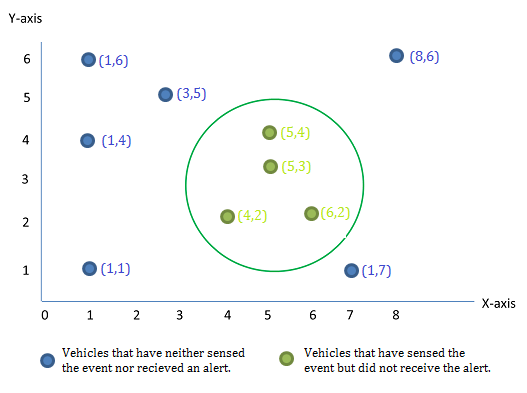
\includegraphics[width=0.5\textwidth]{figs/simulated.png}
    \caption{\name{} event simulation.}
    \label{fig:simulated}
  \end{center}
\end{figure}

%%% Area of Interest overlay
\begin{figure}[ht]
  \begin{center}
    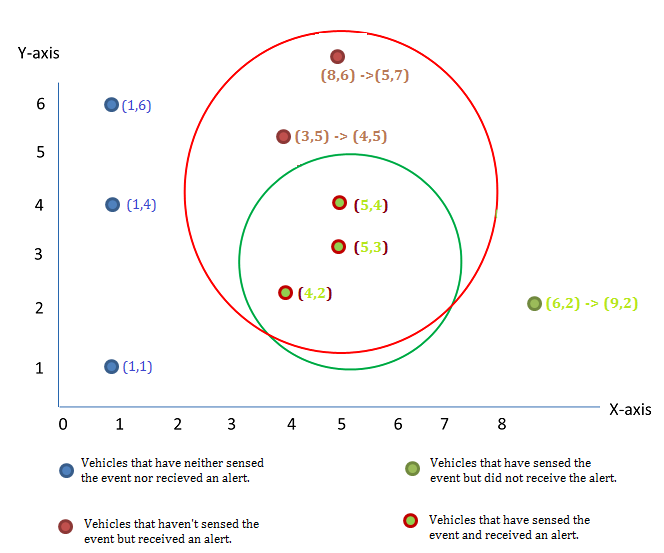
\includegraphics[width=0.5\textwidth]{figs/aoi.png}
    \caption{\name{} Area Of Interest.}
    \label{fig:aoi}
  \end{center}
\end{figure}

By the time AOI message from Message Broker has reached the vehicles
we have observed the vehicle which has sensed the event at location
(6,2) has moved away from the region. This vehicle didn't receive any
alert from \name.  There were two other vehicles that are at
location (3,5) and (8,6) and have moved into the AOI calculated by
Message Broker both these vehicles received the message. And the three
of four vehicles which have sensed the event were still falling within
the Message Broker's AOI and have received an alert.
   
Through this experiment we have verified that all the vehicles within the
AOI of Message Broker have received an alert irrespective of sensing
the event and those vehicles which are out of the AOI did not receive it.

\subsection{Latency Micro-benchmark}

In order to assess the latency response of \name{} under load, we
performed a micro-benchmark involving sending messages at
progressively higher rates, end-to-end. To do this, we developed an
client-side application, ``echorate'', that sends timestamped messages
to the Broker. The Broker responds to these immediately, embedding the
timestamp provided (similar to ICMP ping). The ``echorate'' app takes
rate and total message count as arguments. For this evaluation, we
took baseline measurements at 1 message per second over a one minute
period, then at rates of 10 messages/second up through 1,000
messages/second at roughly logarithmic rate increments. For each increment
we increase the count such that the total test target run time is
10 seconds.

%%% RTT Latency graph
\begin{figure}[ht]
  \begin{center}
    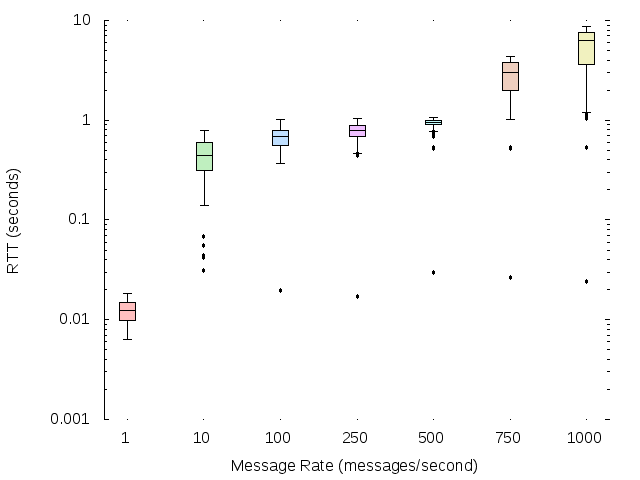
\includegraphics[width=0.5\textwidth]{figs/RTT.png}
    \caption{Round trip time (RTT) as a function of message rate.}
    \label{fig:RTT}
  \end{center}
\end{figure}

The results are presented as a box-and-whisker plot in
figure~\ref{fig:RTT}. Message rate appears as discrete values along
the x-axis. Round trip time is plotted using a log scale on the
y-axis. The dots indicate outliers. This graph shows that the minimum
RTT our prototype manages is about 10 milliseconds. However, even at a
rate of 10 messages/second, the RTT jumps by an order of
magnitude. The response stays fairly flat at around 1 second through a
rate of 500 messages/second. Somewhere between this latter rate and
750 messages/second, the rate begins a linear climb.  This trend is a
result of the \name{} components falling behind in message processing.
As the quartile spread indicates at these higher rates, the RTT slowly
creeps up as message processing continues to lag behind the incoming
message rate.

These results indicate that the prototype needs additional work to
improve its throughput and responsiveness in order to meet the demand
of realistic workloads while maintaining latency-sensitive message
requirements.  Our prototype already uses parallel processing inside
individual components to queue incoming messages.  However, message
processing and sending is single-threaded.  We believe that the key to
increasing throughput is to parallelize these tasks. Decreasing the
RTT baseline message rate can be accomplished by reimplementing
\name{} in a lower-level language where individual processing time
contributions are easier to manage and processing overhead is
generally lower.  Using real-time scheduler directives would likely
also help. We leave such optimizations as future work.

\comment{
\begin{itemize}
\item Discuss evaluation approach.
  \begin{itemize}
  \item Do evaluation in PhantomNet using OpenEPC with emulated RAN.
  \item Use vehicle mobility model, SUMO, to drive realistic mobility scenarios.
  \item Use SUMO output (position, primarily), to trigger handover.
  \end{itemize}
\item Types of evaluations to perform.
  \begin{itemize}
  \item Functional: Endpoints connect and are tracked properly (handover).
  \item Functional: Areas of Interest are interpreted properly.
  \item Scaling: Run simulated/emulated scenarios with dozens of endpoints.
  \item Scaling: Increase message/sec load and observe system response times.
  \end{itemize}
\end{itemize}
}
